\documentclass{article}
\usepackage{lipsum} % Pakiet do generowania sztucznego tekstu
\usepackage{graphicx}

\title{Życie mnie, mnie}
\author{Autor Nieznany}
\date{\today}

\begin{document}

\maketitle

\begin{abstract}
    To jest streszczenie pracy. Lorem ipsum dolor sit amet, consectetur adipiscing elit. Nullam sit amet justo vel libero feugiat feugiat. Pellentesque habitant morbi tristique senectus et netus et malesuada fames ac turpis egestas. Sed nec quam ac metus venenatis consequat.
\end{abstract}

\tableofcontents

\section{Wprowadzenie}
\lipsum[1]

\section{Pierwszy Rozdział}
\subsection{Podrozdział}
\lipsum[2-4]

\section{Drugi Rozdział}
\subsection{Podrozdział}
\lipsum[5-7]

\section{Trzeci Rozdział}
\subsection{Podrozdział}
\lipsum[8-15]

\section{Tekst z Formatowaniem}
\textbf{Pogrubienie}, \emph{Kursywa}, $E=mc^2$.
\underline{Podkreslenie}, $E=mc^2$, \textbf{Pogrubienie}.

\section{Matematyka}
Równanie matematyczne:
\begin{equation}
    \int_{0}^{\infty} e^{-x^2} \, dx = \frac{\sqrt{\pi}}{2}
\end{equation}

\section{Rysunki}
\begin{figure}[h]
    \centering
    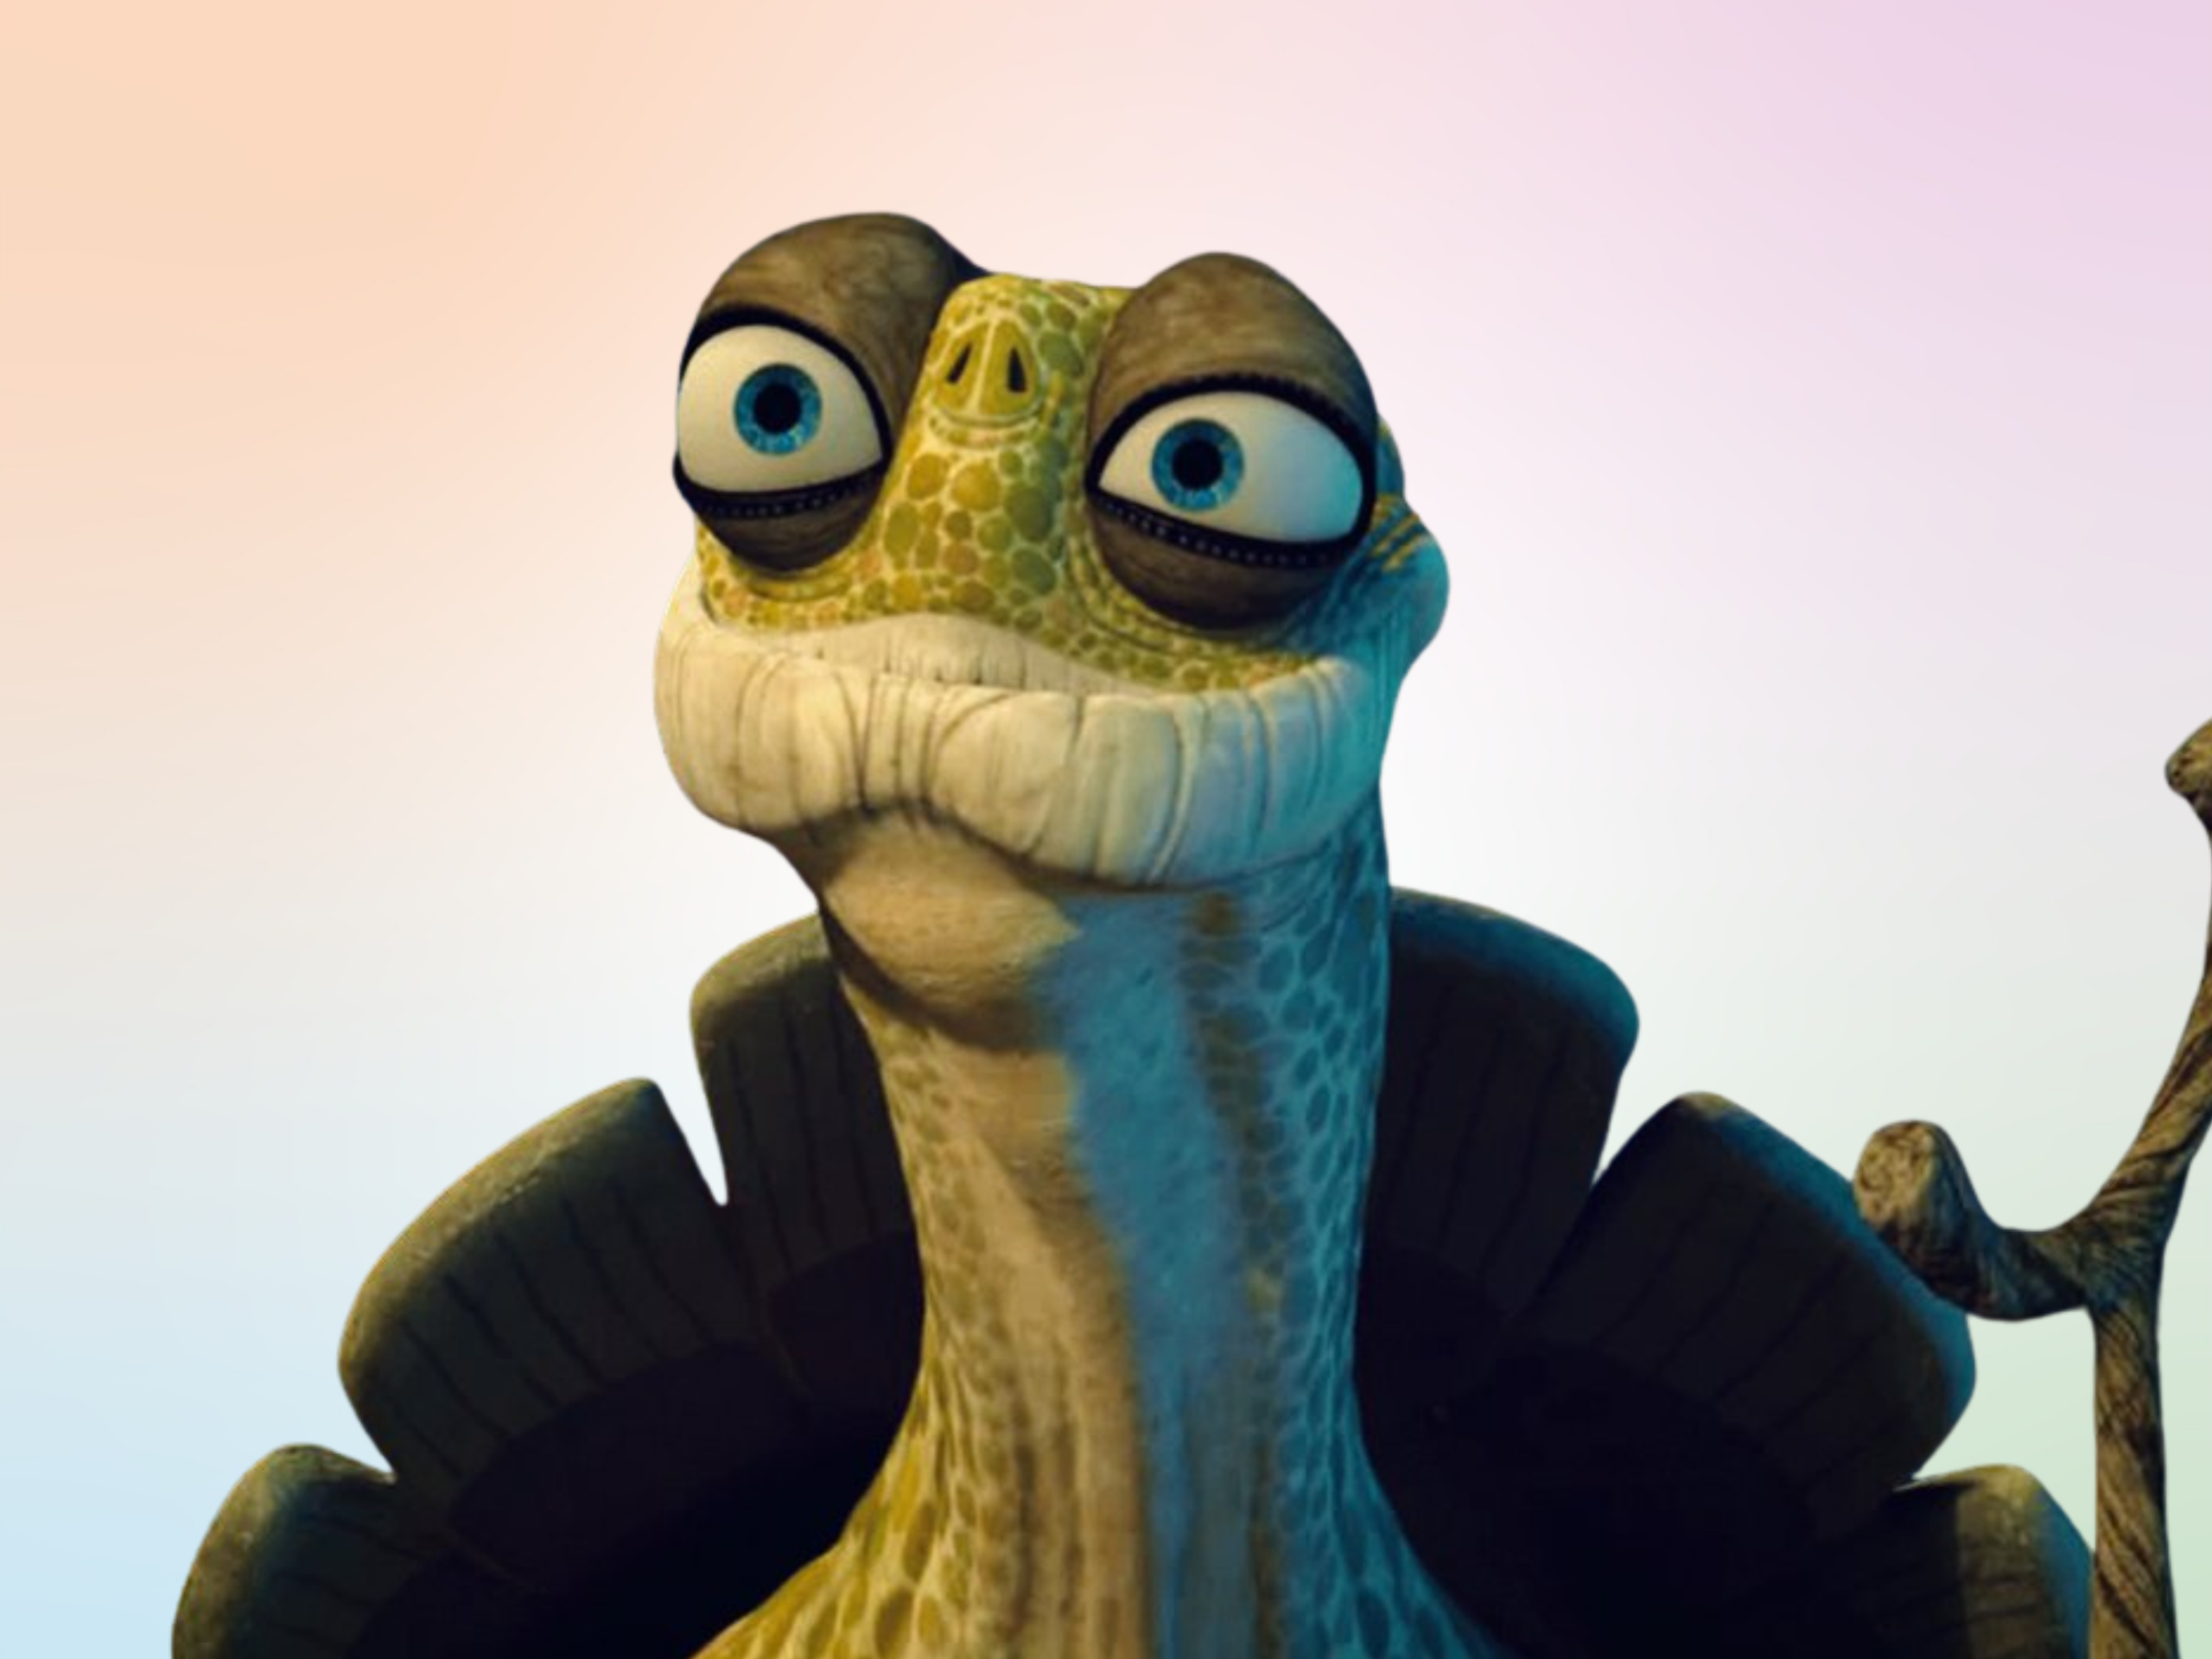
\includegraphics[width=0.5\textwidth]{rysunek1.png}
    \caption{Oogway.}
    \label{fig:rysunek1.png}
\end{figure}

\begin{figure}[h]
    \centering
    \begin{minipage}{0.45\textwidth}
        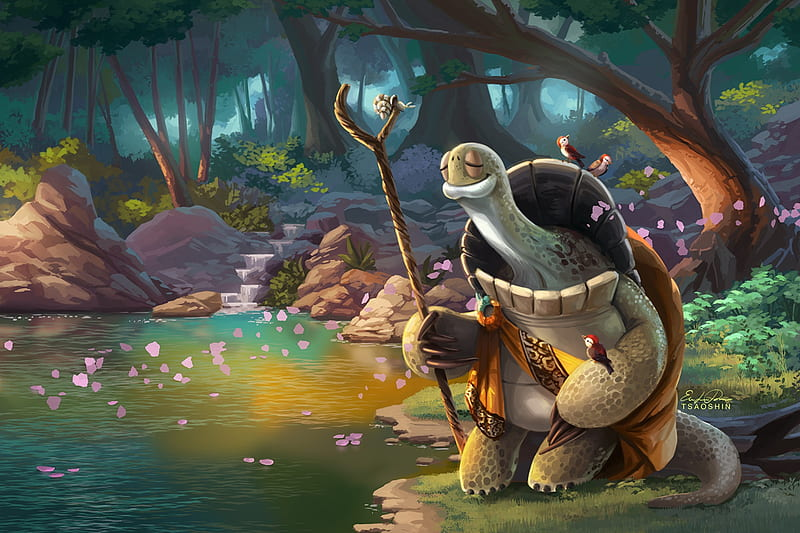
\includegraphics[width=\textwidth]{rysunek2.png}
        \caption{Oogway.}
    \end{minipage}
    \hfill
    \begin{minipage}{0.45\textwidth}
        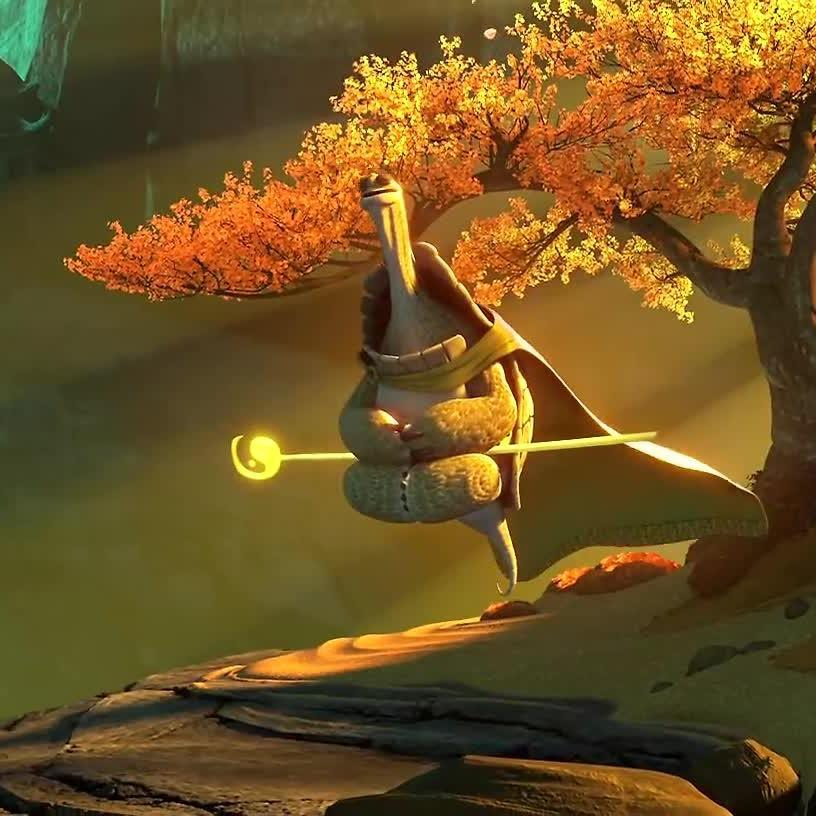
\includegraphics[width=\textwidth]{rysunek3.png}
        \caption{Oogway.}
    \end{minipage}
\end{figure}

\section{Tabela}
\begin{table}[h]
    \centering
    \begin{tabular}{|c|c|}
        \hline
        Kolumna 1 & Kolumna 2 \\
        \hline
        Wartość 1 & Wartość 2 \\
        \hline
        Wartość 3 & Wartość 4 \\
        \hline
    \end{tabular}
    \caption{Tabela odnosząca się do tekstu.}
    \label{tab:tabela1}
\end{table}

\section{Odwołania}
Odniesienie do Rysunku \ref{fig:rysunek1.png}, Tabeli \ref{tab:tabela1}, oraz równania (1).

\section{Podsumowanie}
Lorem ipsum dolor sit amet, consectetur adipiscing elit. Nullam sit amet justo vel libero feugiat feugiat.

\begin{thebibliography}{9}
    \bibitem{autor1} Autor Nieznany. \emph{Eeeeei}. Operon, 2003
    \bibitem{autor2} Jar Jar Binks. \emph{Jedi}. Czarnekowe, 5002 BC
\end{thebibliography}

\end{document}
